\documentclass[../main.tex]{subfiles}

\graphicspath{{\subfix{../images/}}}

\begin{document}

\section{Part 2 - Measurements}

\subsection{Task 1: VCC/GND bounce 1 output}

Remove jumper J1 (“Output 1y1-4 enable (QFN)”), J4 (“Output 1y1-4 enable (SOIC)”) and J9 (“CLK fanout 1G enable”).
\vspace{10pt}
Consult the circuit diagram – which channel (output) is now active on Driver QFN and Driver SOIC? Connect probe 2 to the active output probe point, and confirm the waveform is as expected. Use probe 2 as a trigger signal.
\vspace{10pt}
Confirm that jumper J3(“Bounce sense to GND(QFN)”) is in place. Connect probe 1 to P39(“VCC/GND bounce QFN”) and measure the ground bounce:

\solution

The measurement of the ground and VCC bounce for the QNF- and SOIC packages with one \(\textit{1}\) active output is shown in Figure \ref{fig:gnd_vcc_output_1}. The results are summarized in Table \ref{tab:output_1}.

\begin{figure}[H]
    \centering
    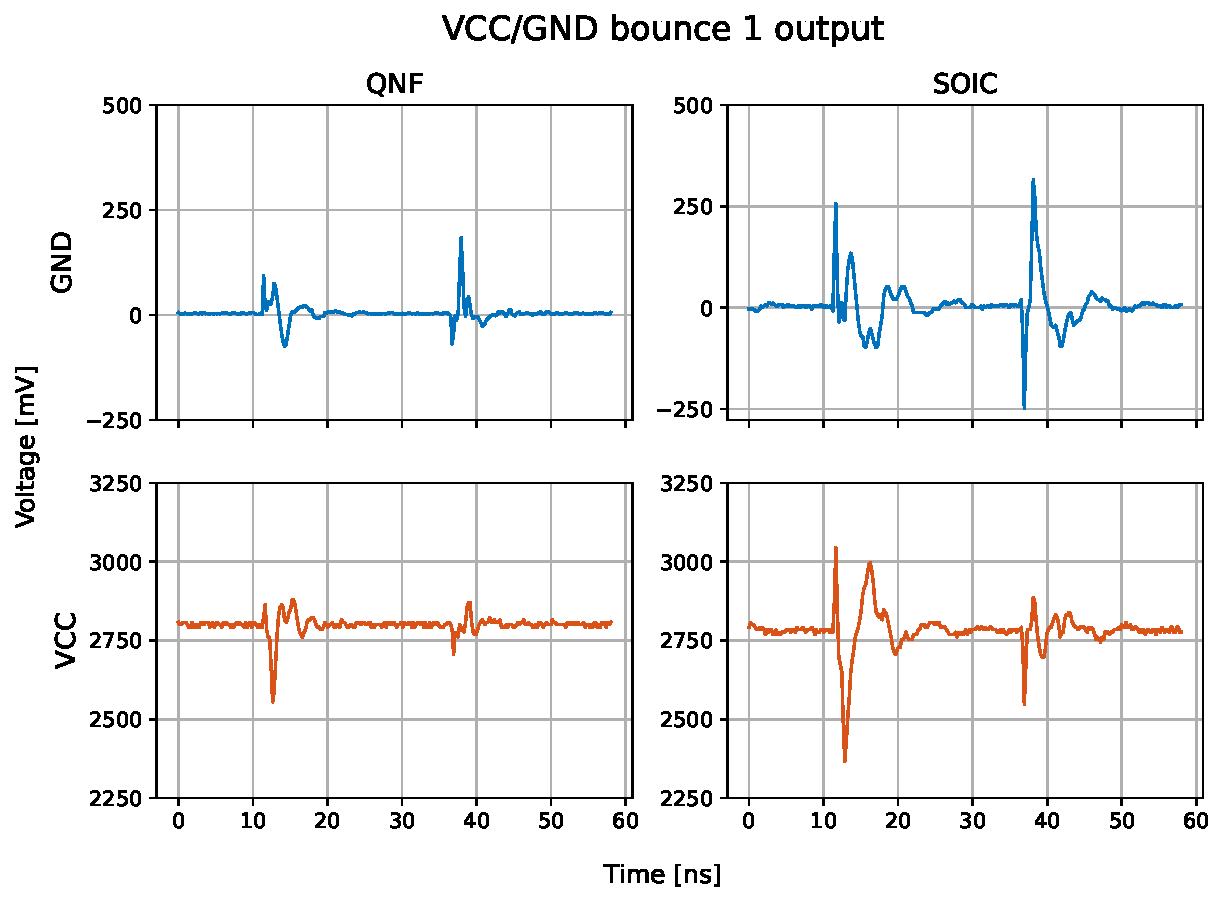
\includegraphics[width=0.8\textwidth]{output_1.pdf}
    \caption{GND and VCC bounce for QNF- and SOIC packages with one \(\textit{1}\) active output.}
    \label{fig:gnd_vcc_output_1}
\end{figure}

\begin{table}[H]
    \centering
    \begin{tabular}{l | r r}
        \toprule[1pt]
        Package type    & GND [mV]  & VCC [mV]\\
        \midrule
        QFN             & 0         & 0  \\
        SOIC            & 1         & 1  \\
        \bottomrule[1pt]
    \end{tabular}
    \caption{GND and VCC bounce for QFN and SOIC packages with one \(\textit{1}\) active output.}
    \label{tab:output_1}
\end{table}

\textbf{Acceptable?}

\subsection{Task 2: VCC/GND bounce 3 outputs}

Place jumper J1 (“Output 1y1-4 enable (QFN)”), J4 (“Output 1y1-4 enable (SOIC)”). Ensure J9 (“CLK fanout 1G enable”) is removed, and that J8(“CLK fanout 2G enable”) is in place.
\vspace{10pt}
Consult the circuit diagram – which channel (output) is now active on Driver QFN and Driver SOIC? Connect probe 2 to the active output probe point, and confirm the waveform is as expected. Use probe 2 as a trigger signal.
\vspace{10pt}
Confirm that jumper J3(“Bounce sense to GND(QFN)”) is in place. Connect probe 1 to P39(“VCC/GND bounce QFN”) and measure the ground bounce:

\solution

The measurement of the ground and VCC bounce for the QNF- and SOIC packages with three \(\textit{3}\) active output is shown in Figure \ref{fig:gnd_vcc_output_3}. The results are summarized in Table \ref{tab:output_3}.

\begin{figure}[H]
    \centering
    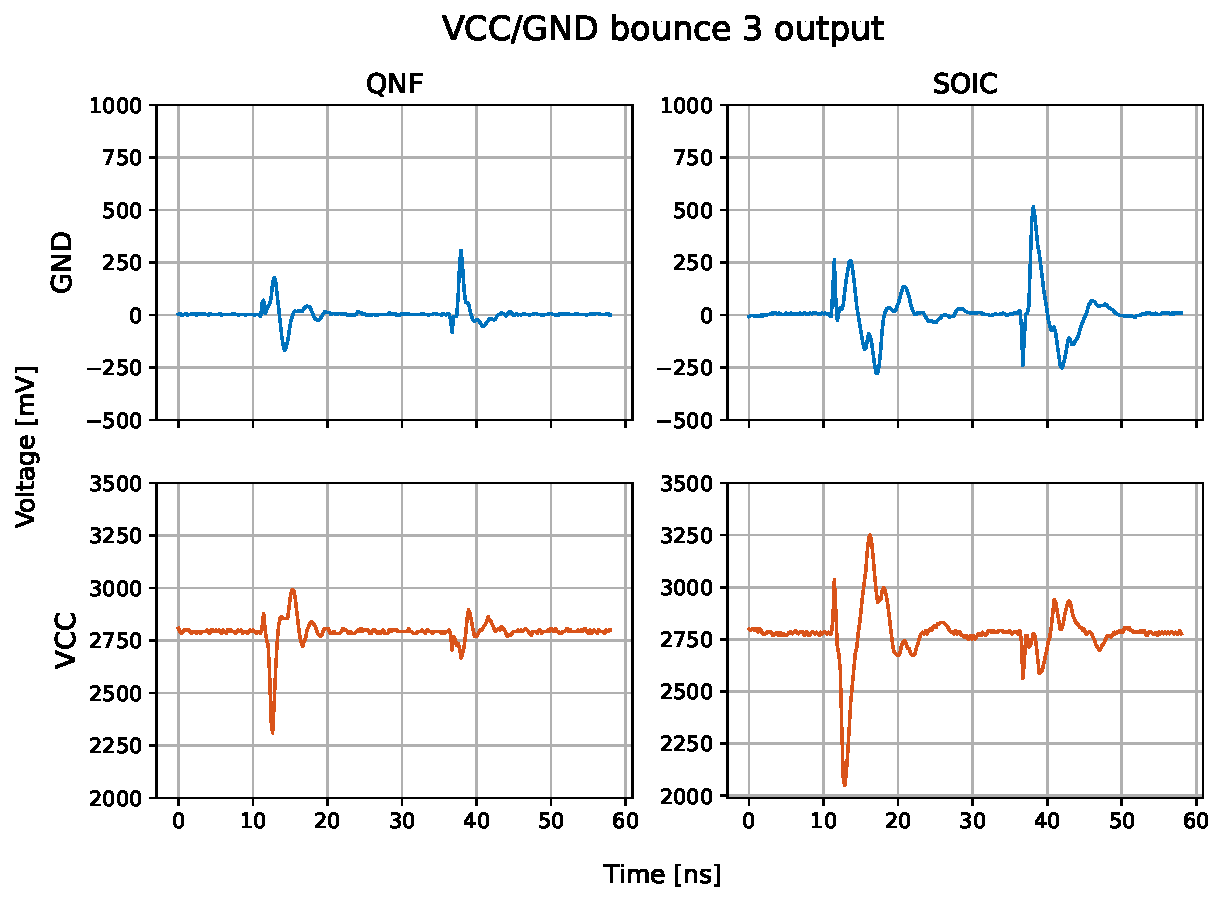
\includegraphics[width=0.8\textwidth]{output_3.pdf}
    \caption{GND and VCC bounce for QNF- and SOIC packages with three \(\textit{3}\) active output.}
    \label{fig:gnd_vcc_output_3}
\end{figure}

\begin{table}[H]
    \centering
    \begin{tabular}{l | r r}
        \toprule[1pt]
        Package type    & GND [mV]  & VCC [mV]\\
        \midrule
        QFN             & 0         & 0  \\
        SOIC            & 1         & 1  \\
        \bottomrule[1pt]
    \end{tabular}
    \caption{GND and VCC bounce for QFN and SOIC packages with three \(\textit{3}\) active outputs.}
    \label{tab:output_3}
\end{table}

\textbf{Acceptable?}

\subsection{Task 3: VCC/GND bounce 7 outputs}

Place all the jumpers on the left. Confirm from the schematic, that all outputs should be enabled.
\vspace{10pt}
Connect probe 2 to the active output probe point, and confirm the waveform is as expected. Use probe 2 as a trigger signal.
\vspace{10pt}
Confirm that jumper J3(“Bounce sense to GND(QFN)”) is in place. Connect probe 1 to P39(“VCC/GND bounce QFN”) and measure the ground bounce:

\solution

The measurement of the ground and VCC bounce for the QNF- and SOIC packages with seven \(\textit{7}\) active output is shown in Figure \ref{fig:gnd_vcc_output_7}. The results are summarized in Table \ref{tab:output_7}.

\begin{figure}[H]
    \centering
    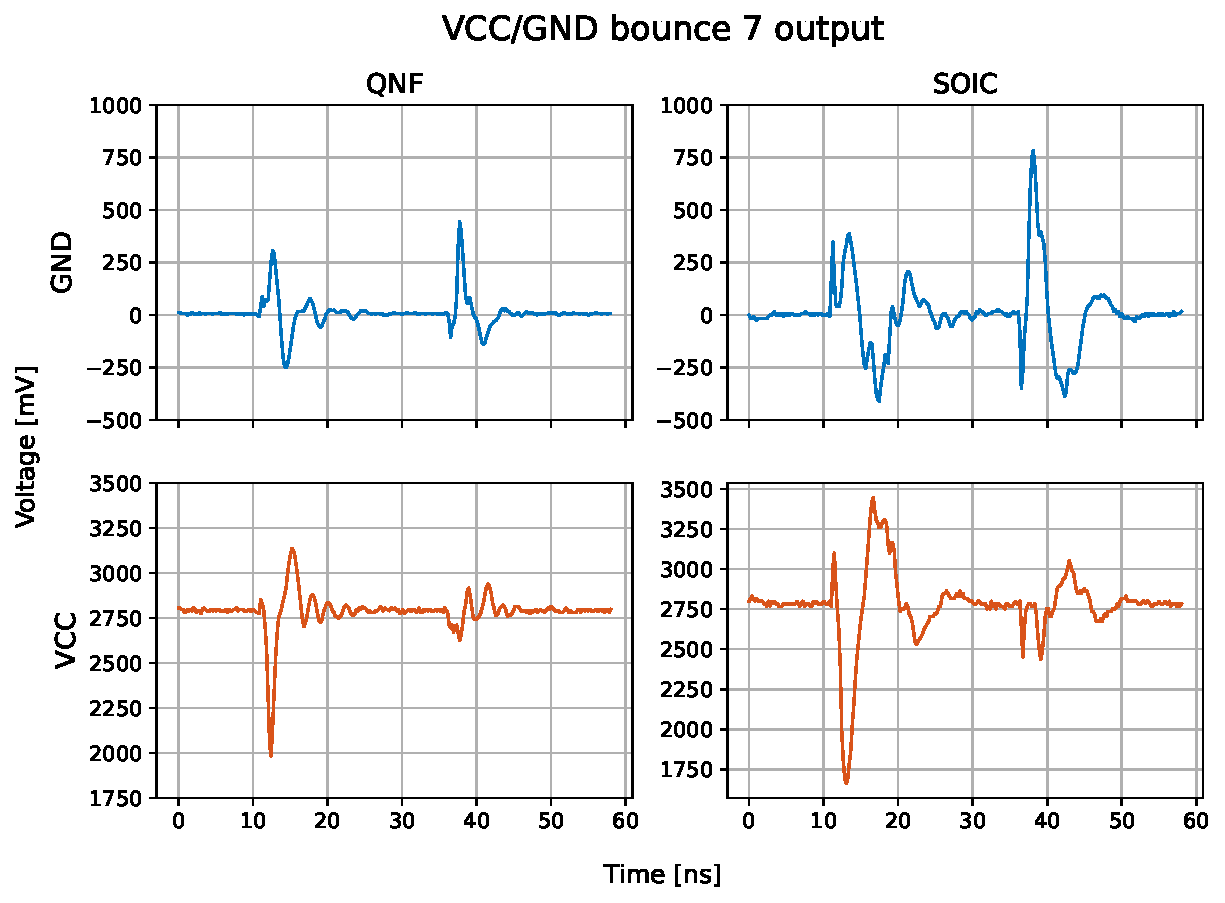
\includegraphics[width=0.8\textwidth]{output_7.pdf}
    \caption{GND and VCC bounce for QNF- and SOIC packages with seven \(\textit{7}\) active output.}
    \label{fig:gnd_vcc_output_7}
\end{figure}
\begin{table}[H]
    \centering
    \begin{tabular}{l | r r}
        \toprule[1pt]
        Package type    & GND [mV]  & VCC [mV]\\
        \midrule
        QFN             & 0         & 0  \\
        SOIC            & 1         & 1  \\
        \bottomrule[1pt]
    \end{tabular}
    \caption{GND and VCC bounce for QFN and SOIC packages with seven \(\textit{7}\) active outputs.}
    \label{tab:output_7}
\end{table}

\textbf{Acceptable?}

\subsection{Task 4: Inverter GND bounce self-oscillation}

Q5 is a hex inverter, SN74ALVC04. The input is a DC voltage set by a potentiometer marked “Inverter VDC input 0-VCC”.
\vspace{10pt}
Confirm that jumper J10 is removed. Only one output on the inverter is active – vary the input using the potentiometer. Can you get the inverter output to oscillate?
\vspace{10pt}
Place jumper J10. All inverter outputs are active – vary the input using the potentiometer. Can you get the inverter output to oscillate? If so, why does it oscillate?

\solution

It was possible to get the inverter output to oscillate when both one and all outputs were active. The oscillations are shown in Figure \ref{fig:inverter_oscillation}. The only noticable differences between the two situations are the amplitude and frequency of the oscillations. %The oscillations are caused by the inverter acting as a ring oscillator.?

\begin{figure}[H]
    \centering
    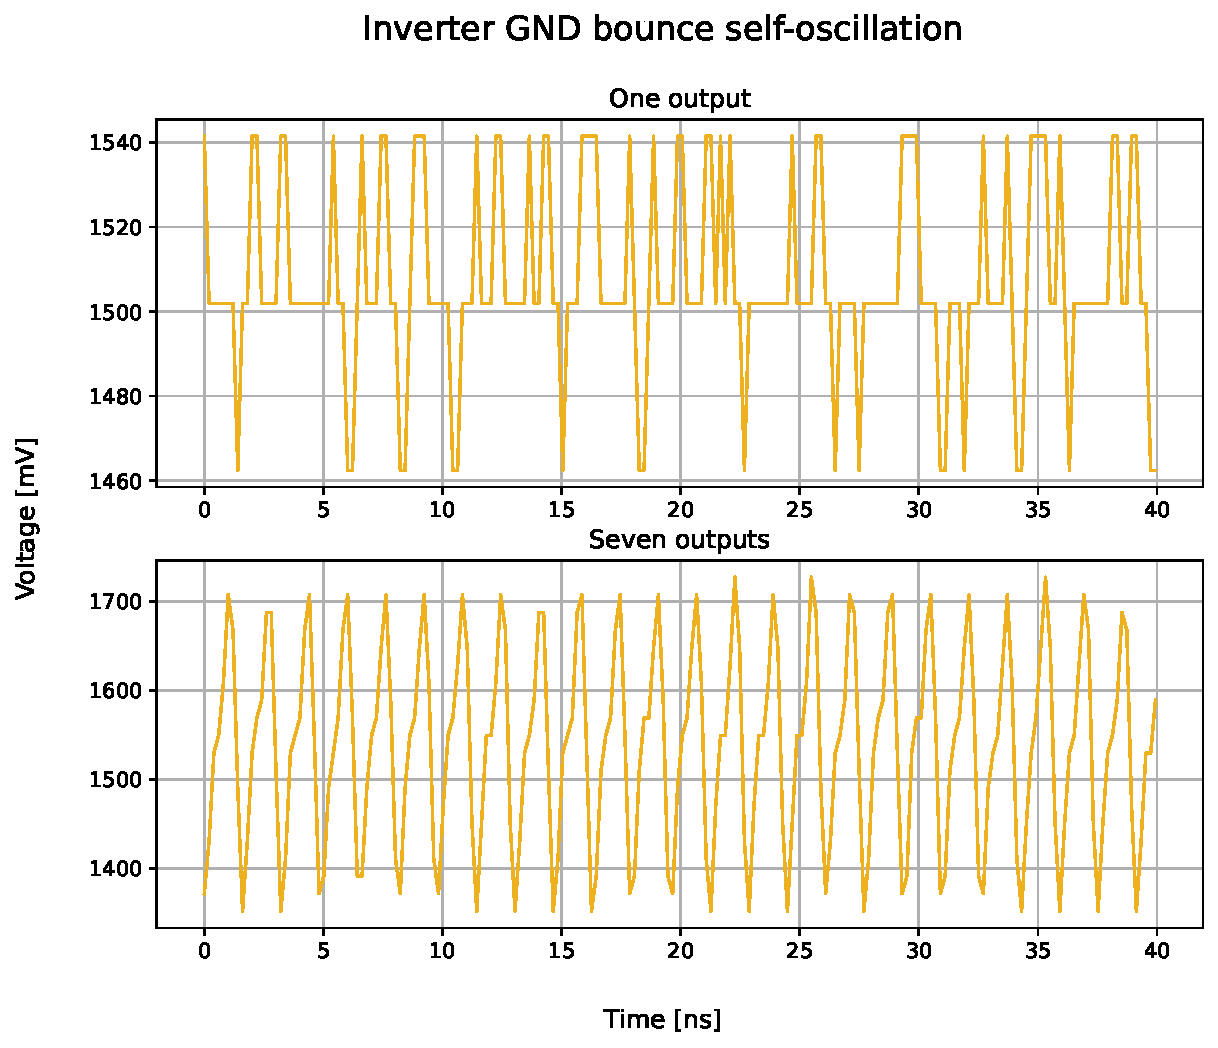
\includegraphics[width=0.8\textwidth]{osci.pdf}
    \caption{Measured oscillations of the inverter output with one and all outputs active.}
    \label{fig:inverter_oscillation}
\end{figure}

\end{document}
